% Explain the implementation of the library rust-debug

% Explain why this library was made.
Retriving the debug infromation from the \emph{DWARF} secionts in the \emph{ELF} file is one of the main problems that needs to be solved when creating a debugger.
The \emph{DWARF} format is made to be space efficent so that the binaryfile dosen't get to large.
This feature of the \emph{DWARF} fomat has a side effect in that it makes it much more complicated for retriving the infromation wanted.
Lukily there exist a library called \emph{gimli-rs} that simplifies reading the \emph{DWARF} format.
But the library still is very complicated to use because it required a lot of knowlage about the \emph{DWARF} format.
Thus the \emph{rust-debug} library was made to simplify this problem even more so that almost no knowlage of the \emph{DWARF} format is needed.


% Explain the overview of the library.
The libarary \emph{rust-debug} is built apone the \emph{gimli-rs} libarary and dosen't restrict the user from accesing the functionality of that libarary.
It uses the \emph{gimli-rs} library for paring the \emph{DWARF} sections into more workable datastructures, the figure \ref{fig:rustdebug} shows how they are connected.
The goal of the desing of the library is that a user should be able to just call a function for retriving debug information such as a stacktrace and at the same time be able to use the \emph{gimli-rs} functionality to retrive the same iformation if wanted.
The library is has the features to retive the call stack, stackframes, variables, sourceinfomaiton and a evalution function for evaluating the values of variables.


\begin{figure}[h]
    \centering
    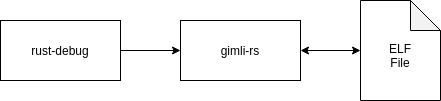
\includegraphics[width=1.0\textwidth]{rust_debug.png}
    \label{fig:rustdebug}
\end{figure}


% Explain the evaluation part. % TODO
% Explain the stored target memory and registers
As mention before one of the requirements for evaluating the value of a variable is access to the registers and memory of the debugee.
This libarary does not have that functionality because the problem of accesing memory and register is out of scope for this library.
The reason being that it would limit the number of systmes it could be used for too the systmes it support and also the goal of this library is to make it simpler to get debug information from \emph{DWARF}, and not to proveide an interface to the systmes memory and register.
That lead to the motivaiton of creating a datastructure that holds these needed values of the system.
The implimitation is just a struct with two hashmaps, one for the memory values and one for the register values.
It also has some metods for retriving the stored values.
This struct is then used as an argument to the functions in the library and if a value that is not pressent in the datastucure is needed the result of the fuction call will be a request ot add the to the datastracure and call the function again.
This has a negative effect in that some of the calucations will be repeated mutiple times but it is not very notesable.


% Explain the evaluation of vairbles.
The libarary has a structur called \emph{VariableCreator} which  takes a refrense to the \emph{DWARF} unit and die of the variable.
Then there is a evalution method that takse the memory and registers data structure and proforms caluclation to evalue and retrive variable information.
This method return an enum that eiter tell the user what memory or reigster valuse are needed, or that the it is done and the method \emph{get\_variable} can be used to get the vairable.
The variable structure continas the name, value, type, sourcelocaiton and the location of where the value was evaluated from.


% Explain the evaluation of call stack % TODO
% Explain the evaluation of stackframe % TODO
% Explain the evaluation of source informaiton % TODo

